%% This is file `elsarticle-template-1-num.tex',
%%
%% Copyright 2009 Elsevier Ltd
%%
%% This file is part of the 'Elsarticle Bundle'.
%% ---------------------------------------------
%%
%% It may be distributed under the conditions of the LaTeX Project Public
%% License, either version 1.2 of this license or (at your option) any
%% later version.  The latest version of this license is in
%%    http://www.latex-project.org/lppl.txt
%% and version 1.2 or later is part of all distributions of LaTeX
%% version 1999/12/01 or later.
%%
%% The list of all files belonging to the 'Elsarticle Bundle' is
%% given in the file `manifest.txt'.
%%
%% Template article for Elsevier's document class `elsarticle'
%% with numbered style bibliographic references
%%
%% $Id: elsarticle-template-1-num.tex 149 2009-10-08 05:01:15Z rishi $
%% $URL: http://lenova.river-valley.com/svn/elsbst/trunk/elsarticle-template-1-num.tex $
%%
\documentclass[preprint,12pt]{elsarticle}
\usepackage{amsmath}
\usepackage{graphicx,subcaption}
\usepackage{listings}
\usepackage{hyperref}
\usepackage{multirow}
\usepackage{notoccite}
\hypersetup{
    colorlinks,
    citecolor=black,
    filecolor=black,
    linkcolor=black,
    urlcolor=black
}

%% Use the option review to obtain double line spacing
%% \documentclass[preprint,review,12pt]{elsarticle}

%% Use the options 1p,twocolumn; 3p; 3p,twocolumn; 5p; or 5p,twocolumn
%% for a journal layout:
%% \documentclass[final,1p,times]{elsarticle}
%% \documentclass[final,1p,times,twocolumn]{elsarticle}
%% \documentclass[final,3p,times]{elsarticle}
%% \documentclass[final,3p,times,twocolumn]{elsarticle}
%% \documentclass[final,5p,times]{elsarticle}
%% \documentclass[final,5p,times,twocolumn]{elsarticle}

%% if you use PostScript figures in your article
%% use the graphics package for simple commands
%% \usepackage{graphics}
%% or use the graphicx package for more complicated commands
%% \usepackage{graphicx}
%% or use the epsfig package if you prefer to use the old commands
%% \usepackage{epsfig}

%% The amssymb package provides various useful mathematical symbols
\usepackage{amssymb}
%% The amsthm package provides extended theorem environments
%% \usepackage{amsthm}

%% The lineno packages adds line numbers. Start line numbering with
%% \begin{linenumbers}, end it with \end{linenumbers}. Or switch it on
%% for the whole article with \linenumbers after \end{frontmatter}.
\usepackage{lineno}
\usepackage{enumitem}

%% natbib.sty is loaded by default. However, natbib options can be
%% provided with \biboptions{...} command. Following options are
%% valid:

%%   round  -  round parentheses are used (default)
%%   square -  square brackets are used   [option]
%%   curly  -  curly braces are used      {option}
%%   angle  -  angle brackets are used    <option>
%%   semicolon  -  multiple citations separated by semi-colon
%%   colon  - same as semicolon, an earlier confusion
%%   comma  -  separated by comma
%%   numbers-  selects numerical citations
%%   super  -  numerical citations as superscripts
%%   sort   -  sorts multiple citations according to order in ref. list
%%   sort&compress   -  like sort, but also compresses numerical citations
%%   compress - compresses without sorting
%%
%% \biboptions{comma,round}

% \biboptions{}

\let\originaleqref\eqref
\renewcommand{\eqref}{Eq.~\originaleqref}

\hypersetup{colorlinks=true,
  pdftitle={Brightness of the liquid determium cold source measured from the ICON beamline at the Swiss Spallation Neutron Source (SINQ)},
  pdfauthor={Ryan M. Bergmann, Masako Yamada, Tibor Reiss, Michael Wohlmuther, Uwe Filges}}

\journal{Nuclear Instruments and Methods in Physics Research Section A: Accelerators, Spectrometers, Detectors and Associated Equipment}

\begin{document}

\begin{frontmatter}

%% Title, authors and addresses

%% use the tnoteref command within \title for footnotes;
%% use the tnotetext command for the associated footnote;
%% use the fnref command within \author or \address for footnotes;
%% use the fntext command for the associated footnote;
%% use the corref command within \author for corresponding author footnotes;
%% use the cortext command for the associated footnote;
%% use the ead command for the email address,
%% and the form \ead[url] for the home page:
%%
%% \title{Title\tnoteref{label1}}
%% \tnotetext[label1]{}
%% \author{Name\corref{cor1}\fnref{label2}}
%% \ead{email address}
%% \ead[url]{home page}
%% \fntext[label2]{}
%% \cortext[cor1]{}
%% \address{Address\fnref{label3}}
%% \fntext[label3]{}

\title{Brightness of the liquid determium cold source measured from the ICON beamline at the Swiss Spallation Neutron Source (SINQ)}

%% use optional labels to link authors explicitly to addresses:
%% \author[label1,label2]{<author name>}
%% \address[label1]{<address>}
%% \address[label2]{<address>}

\author{Ryan M. Bergmann\corref{rmb}}
\ead{ryan.bergmann@psi.ch}
\cortext[rmb]{Corresponding author. Tel.: +41.56.310.56.12.}

\author{Masako Yamada}
%\ead{masako.yamada@psi.ch}


\author{Tibor Reiss}
%\ead{tibor.reiss@psi.ch}

\author{Michael Wohlmuther}
%\ead{michael.wohlmuther@psi.ch}

\author{Uwe Filges}
%\ead{uwe.filges@psi.ch}



\address{Paul Scherrer Institut, Villigen, Switzerland}

\begin{abstract}


\end{abstract}

\begin{keyword}
brightness \sep cold


\end{keyword}


\end{frontmatter}

\linenumbers

%% main text

\section{Introduction}
\label{sec:intro}

The Swiss Spallation Neutron Source (SINQ) is a spallation neutron source driven by a continuous 590 MeV proton beam at the Paul Scherrer Institut in Villigen, Switzerland.  The incoming protons impinge on a lead target cooled with heavy water, producing high energy neutrons.  These neutrons are moderated by the tank of D$_2$O surrounding the target.  The cold source is a 20 liter volume of liquid D$_2$ at approximately 25 K located within the D$_2$O moderator tank with its innermost face approximately 35 cm away from the center of the target.  It serves to further reduce the energies of the ``thermal'' neutrons coming from the D$_2$O tank into a regime that is more useful to instruments which receive neutrons from its surface.  

There is an extended shutdown of SINQ ambitiously planned for 2018 which will provide an opportunity for changes to be made to the cold neutron source \cite{rueegg_icans}.  Any changes will require a large amount of calculations done to minimize risk and ensure good the proposed changes will benifit the facility and its users.  The brightness measureemtn presented in this paper is the first step in validating the computational models reuqired to carry out a sucessful upgrade.  

The brightness measurement was conducted on July 21, 2014 in the ICON beamline at SINQ.  ICON is the cold neutron imaging facility at the neutron spallation source SINQ. The beamline offers an aperture wheel to change beam intensity and collimation ratio, as well as large evaculated flight tubes to minimize losses from scattering in the air \cite{icon}.  ICON was chosen since it does not incorporate any neutron optics, has good collimation, and looks directly on the surface of the cold source.  This removes additional uncertainty associated with the current state of the neutron guides and the physics involved with neutron-refecltive surfaces.

\section{Experimental Setup}
\label{sec:setup}

The layout of the experimental is shown in Figure \ref{fig:geom}, which is a horizonal cut of the MCNP model geometry.  The target and moderators are shown furthest to the right.  The vertical line is the shielding monolith boundary, which is mostly steel blocks.  The ICON bunker is to the left of the monolith, the walls of which are made of heavy concrete and are shown as rectangular blocks.  The velocity selector that is usually mounted on the monolith wall in the ICON bunker was removed for this measurement.

\begin{figure}[h!] 
  \centering
    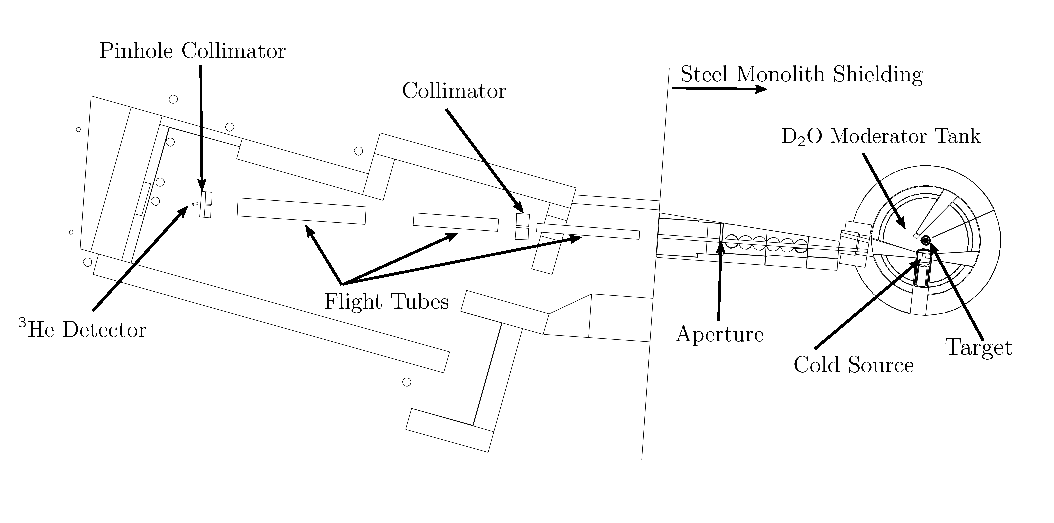
\includegraphics[width=\textwidth]{graphics/geom_bw_labels.eps}
     \caption{Geometry \label{fig:geom} }
\end{figure}

Figure \ref{fig:det} shows a photograph of the $^3$He detector with the iron pinhole collimator positioned in front of it before the large shielding blocks and sapphire crystals were positioned.

\begin{figure}[h!] 
  \centering
    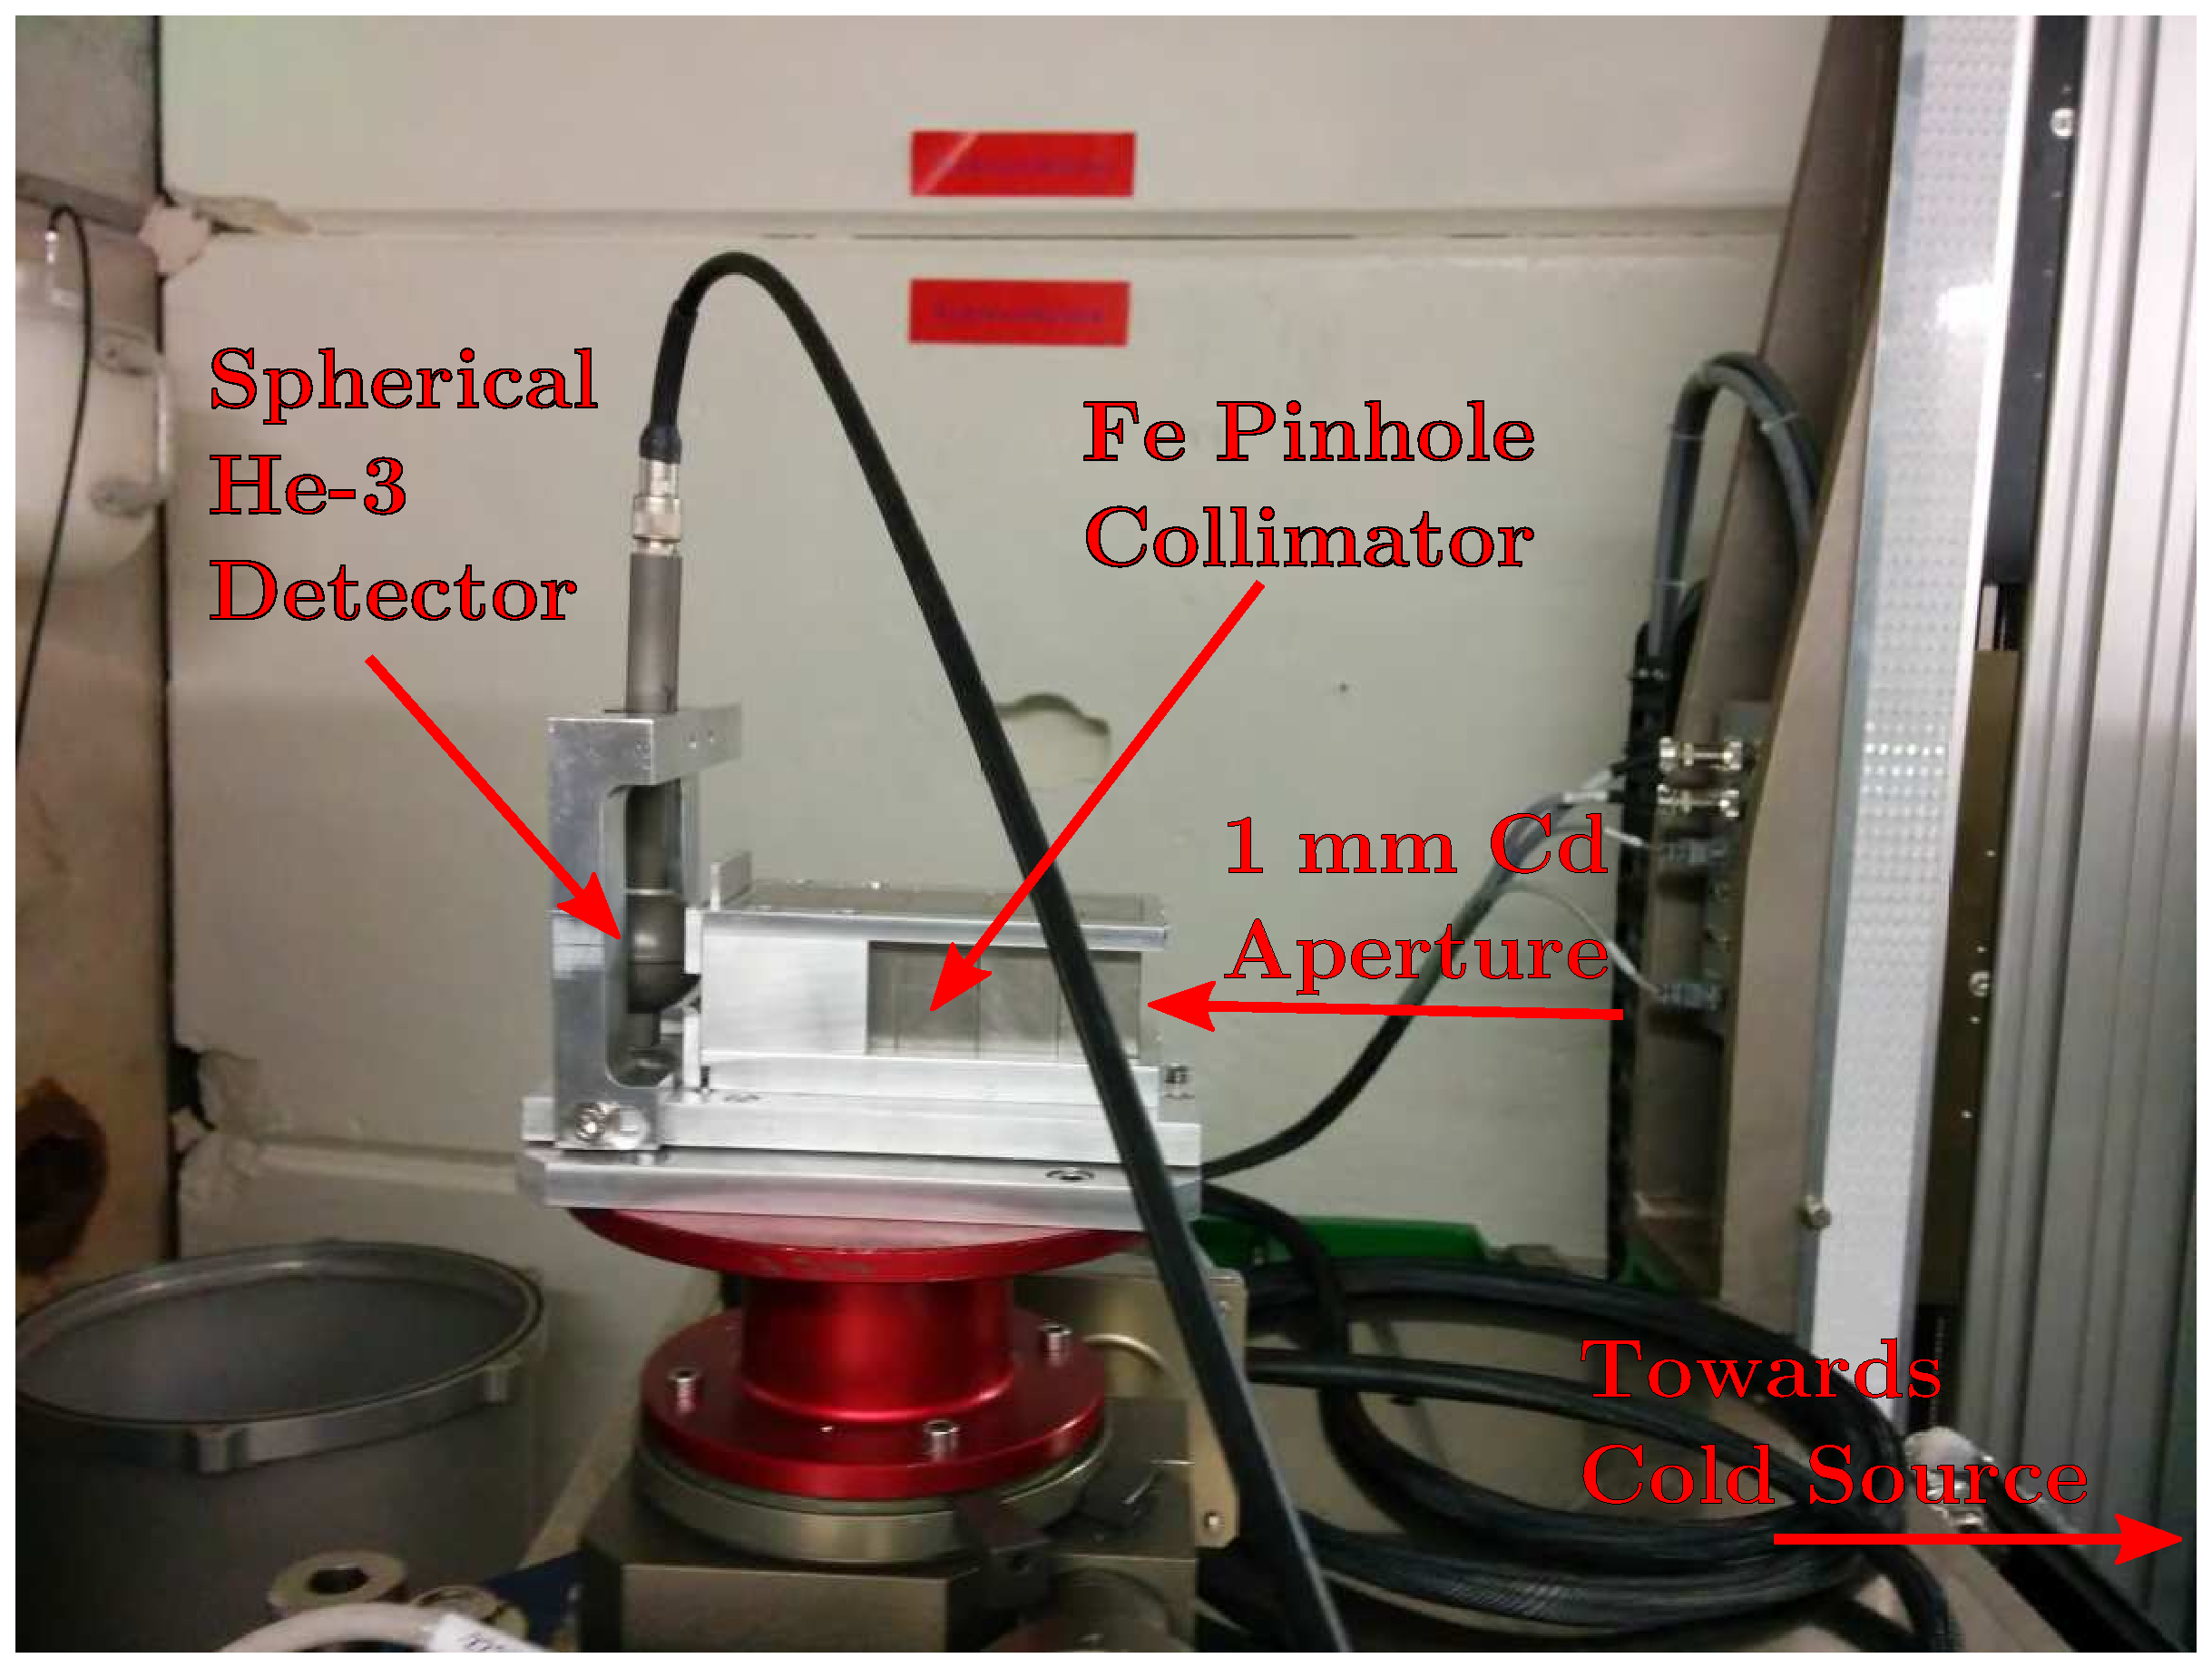
\includegraphics[width=\textwidth]{graphics/det.eps}
     \caption{$^3$He detector with iron collimator. \label{fig:det}}
\end{figure}

The principle components in the neutron path, listed in increasing distance from the detector during the measurement, were:

\begin{center} \underline{In-bunker components}\end{center}
\begin{enumerate}
  \item Spherical $^3$He detector, 3.30 cm $\oslash$, sorrounded by 1 mm cadmium sheets on all sides except towards the pinhole collimator
  \item Cadmium aperture, 1 mm $\oslash$, 1 mm thick, 1 mm from the detector surface
  \item Iron pinhole collimator, 100 mm long, immediately after the cadmium aperture, surrounded by heavy concrete, lead, and polyethylene shielding
  \item Sapphire crystals, 20x20 mm faces, 80 mm total thickness, within the heavy concrete, lead, and polyethylene shielding
  \item Evacuated flight tubes with 1.0 mm thick aluminum faces, ~7410 mm total length 
  \item Steel collimator, 50x50 mm aperature 7548 mm from detector
\end{enumerate}
\begin{center}\underline{In-pile components}\end{center}
\begin{enumerate}[resume]
  \item Moveable gadolinium circular aperature wheel, set to the largest opening of 80 mm $\oslash$
  \item High energy shutters
  \item Zapfen unit, 40x120 mm
  \item D$_2$O moderator tank
  \item Low pressure nozzle which pentrates the D$_2$O moderator tank, end size is 138x138 mm
  \item Liquid deuterium cold source
  \item Lead spallation target
\end{enumerate}


Since brightness/brilliance was to goal of the measurement, the solid angle seen by the detector is needed to normalize the spectra.  The cadmium sheet limits the sensitive region of the helium detector to a 1 mm diameter circle, and the the other items in the beam path create a system that limited the angular view of the detector.  Table \ref{tab:sa} shows the maximum solid angle of the various items in the neutron beam.  The values are the minimum of the item's self-collimation (due to its thickness) and the collimation of the system formed by the item and the hole in the cadmium sheet.  Figure \ref{fig:solid_angle} shows a cartoon of the collimation system formed by the items and the cadmium hole.

\begin{figure}[h!] 
  \centering
    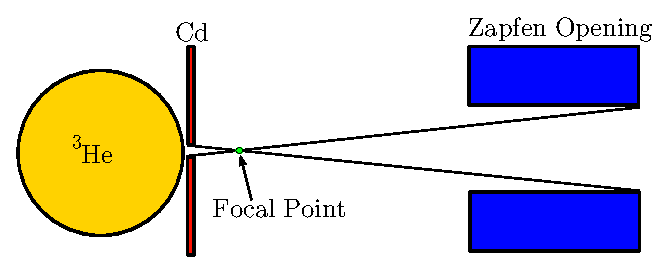
\includegraphics[width=\textwidth]{graphics/solid_angle.eps}
     \caption{The limiting collimation system in the measurement in the horizontal plane (not to scale), and the crossing point where the point detector was place in the MCNP simulations. \label{fig:solid_angle}}
\end{figure}

\begin{table}
\begin{center}
     \caption{Table of solid angles with the limiting member marked with boldface and a star (*).  \label{tab:sa} }
\begin{tabular}{|l|r|r|r|}
     \hline
                   &     Horizontal  &     Vertical   &     Diagonal   \\
     \hline
     Fe Collimator &     6.9282E-04  &     6.9282E-04 &     6.9282E-04 \\
     \hline 
     Cadmium Hole  &     1.8403E-00  &     1.8403E-00 &     1.8403E-00 \\
     \hline 
     Sapphire      &     1.9781E-03  &     1.9781E-03 &     3.8449E-03 \\
     \hline 
     Steel         &     3.3167E-05  &     3.3167E-05 &     6.5574E-05 \\
     \hline
     Aperture      &     3.4016E-05  &     3.4016E-05 &\bf* 3.4016E-05 \\
     \hline
     Tube          &     2.2597E-05  &\bf* 2.2597E-05 &    4.4867E-05  \\
     \hline
     Zapfen        &\bf* 2.0707E-05  &     4.6208E-05 &     6.6559E-05 \\
     \hline
     Nozzle        &     5.1293E-05  &     5.1293E-05 &     1.0215E-04 \\
     \hline
\end{tabular}
\end{center}
\end{table}

It can be seen that in the horizontal plane, the Zapfen opening (where the beamline opens into large nozzle in the moderator tank) is the limiting item.  In the vertical plane, the limiting item is the steel shielding blocks positioned before the chopper.  At 45 degrees, the aperture wheel is the limiting case.  These items are shown in the pinhole image calculated with MCNP and discussed in Section \ref{sec:sim}.

\section{Simulations and Solid Angle}
\label{sec:sim}

Simulations were done with MCNP6.1 and with ENDF/B-VII.1 data.  Thermal scattering data for the room temperature sapphire crystals were used \cite{sapp}, as were 77 K thermal scattering data for beryllium, 19 K data for ortho-/para-deuterium, 273 K data for heavy water, 273 K data for light water \cite{mcnp6}, and 25 K data for aluminum, and 25 K data for zirconium \cite{IKE}.  The aliumun and zirconium data are important for accurately simulating the transmission through the various hulls surrounding the deuterium in the cold source.  The model geometry of has already been shown in Figure \ref{fig:geom}, and was created to be as true-to-life as possible.  The target in use during the measurement was ``target 10'', which is shown in Figure \ref{fig:target}. This target had a hemispherical beam entrance window, STIP samples, and some light water contamination in the inner cooling loop.  These features were modelled in the MCNP simulation \cite{target10}.

\begin{figure}[h!] 
  \centering
    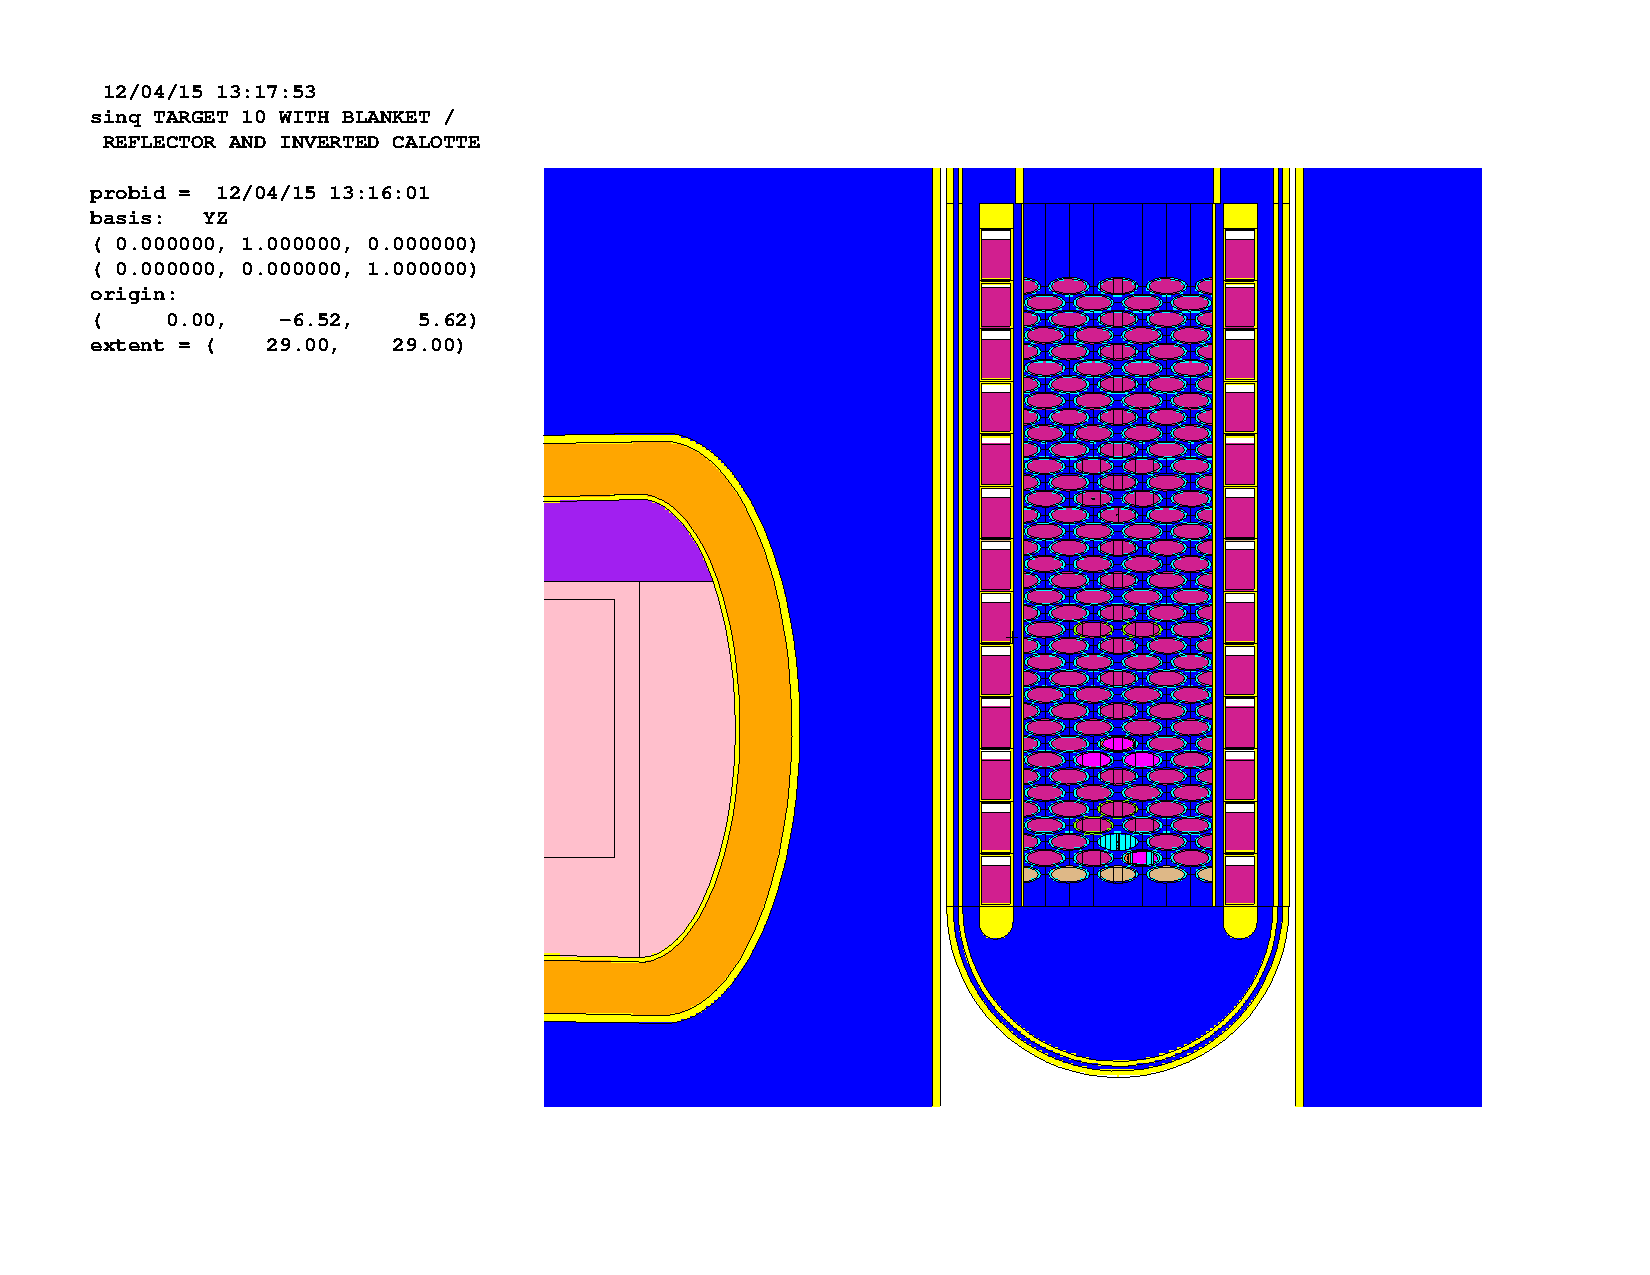
\includegraphics[width=0.25\textwidth,trim={15cm 0 5cm 0},clip]{graphics/target.pdf}
     \caption{Vertical cross section of the target MCNP model geometry. \label{fig:target}}
\end{figure}

Since the detector is very far away from the neutron source, special methods had to be used in order to gather sufficient statistics in a reasonable amount of time.  A point detector is a ``next event'' estimator that scores a tally at every neutron collision event \cite{mcnp}.  The contribution to the tally is weighted by the probability of the neutron scattering into the direction of the detector point and travelling to the detector without colliding again (i.e. weight is rediced by the attentuation of the material in between).  

Using a point detector would be a reasonable solution if only cancluated the flux was desired, but the brightness also depends on the view able solid angle of the detector system.   The physical system responds to a view limited by the pinhole collimator and cadmium sheet, which produces a small, finite spot on detector surface.  A regular point detector would only see a single point of this view and wouldn't report any angular information needed for caluclating the brightness.  If the point detector were placed at the crossing point of the collimation system, it would see the full flux visible to the detector, but it would summed over all angles.  In order to calculate the solid angle visible, a ``pinhole radiography tally'' was used in MCNP.  This tally calculates contributions in the same way, but it projects the contibutions through the point onto an image plane.  If such a projection is placed behind all the items which limit the detector view, the solid angle visible to the detector can be calculated by summing the solid angle each pixel corresponds to.

Figure \ref{fig:pinhole_image} shows a pinhole radiography tally image generated at the upstream surface of the cadmium sheet with the pinhole placed at the horizontal collimation crossing point.  The Zapfen limits the view on the horizontal plane, so the hole in the cadmium lines up perfectly with projection of the Zapfen.  The other limiting objects are also projected onto the plane to show the planes where they limit the detector view.

\begin{figure}[h!] 
  \centering
    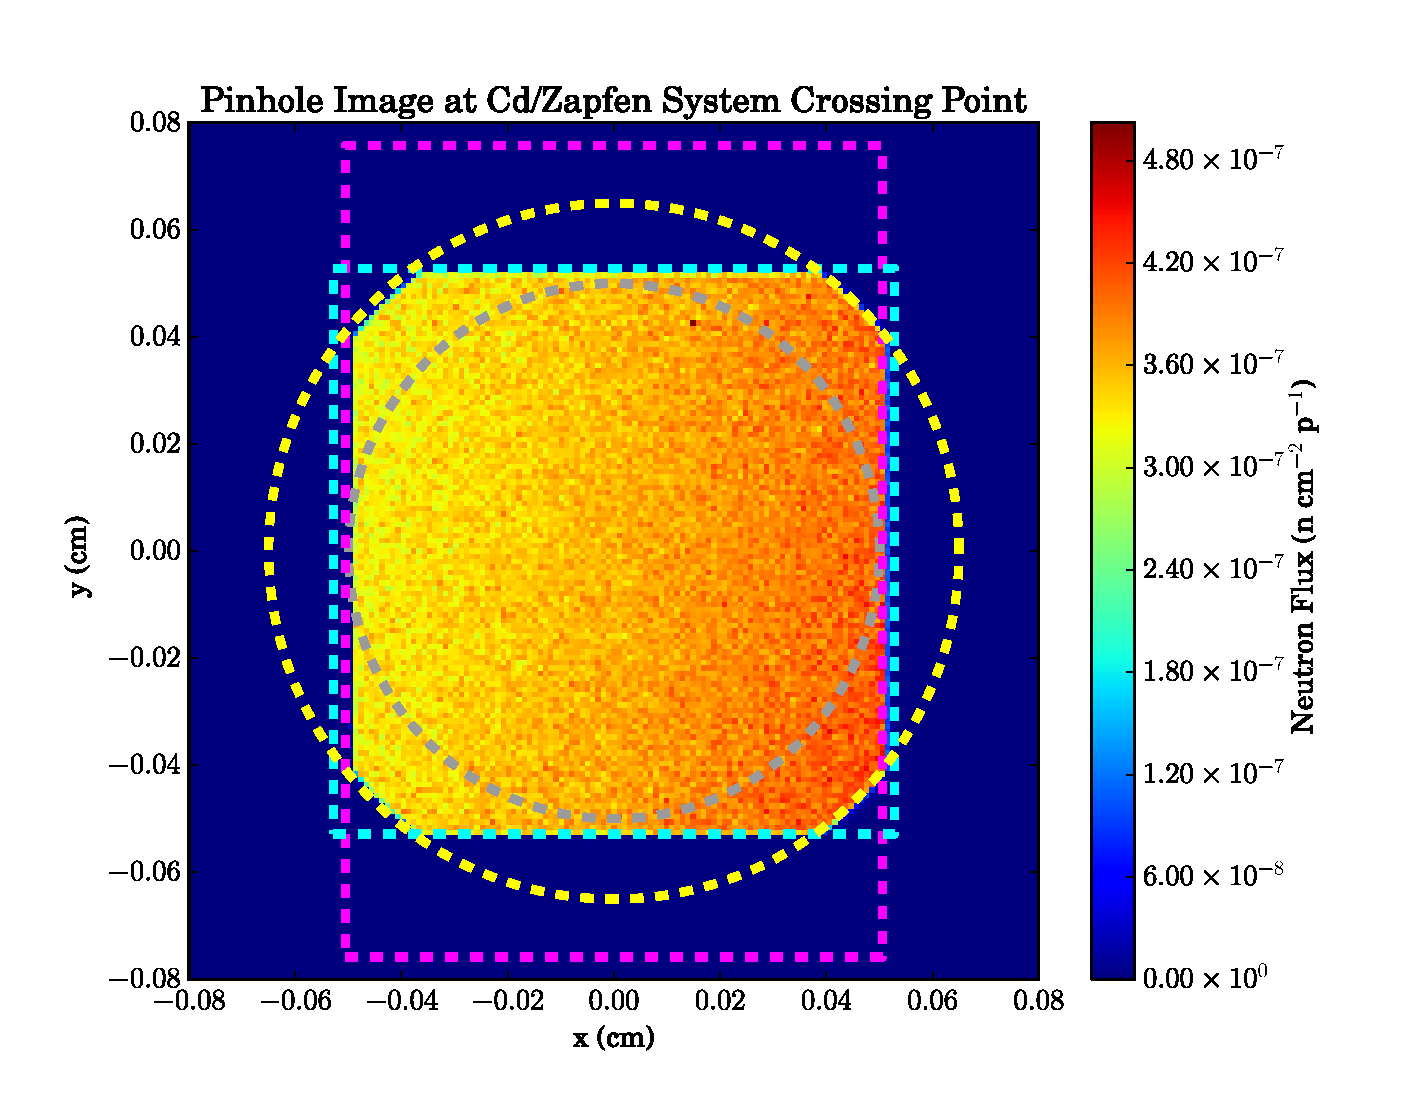
\includegraphics[width=\textwidth]{graphics/pinhole.eps}
     \caption{The flux image created by a pinhole radiography tally in MCNP at the collimation crossing focal point.  The image plane is at upstream surface of the cadmium sheet.  The outlines show the projections of the limiting geometry through the pinhole: Grey=cadmium hole, blue=beam port, magenta=Zapfen, yellow=Gd aperture. \label{fig:pinhole_image}}
\end{figure}

From this image, it was deduced that the total solid angle visible to the detector was limited to $2.1363\times10^{-5}$ steradians.  

The hole is fully illuminated (there are no spots on the where a radiography tally produced a zero result), so the area used to normalize the spectra is the area of the hole (7.85398$\times 10^{-3}$ cm$^2$).



\section{Detector Efficiency}
\label{subsec:eff}

The efficiency curve of the helium detector was also measured and compared to calculated curves.  Curves were calculated using a 1D model and 1/v cross sections as well as with a detailed MCNP model of the helium detector \cite{bonner_manual}.  The 1D model efficiency is shown in Eq. \ref{eqn:eff1}, where $\Sigma_{\textrm{stl}}$ is the stainless steel total macroscopic cross section, $\Sigma_{\textrm{He}}$ is the $^3$He absorbtion macroscopic cross section, $x_{\textrm{stl}}$ is the thickness of the detector's stainless steel shell, and  $D_{\textrm{stl}}$ is the diameter $^3$He volume.  The cross section wavelength dependence is shown in Eq. \ref{eqn:eff2}, where $a$ and $b$ are linear fit coefficients derived from cross section data.  

\begin{gather}
     \label{eqn:eff1} \epsilon(\lambda) = \exp \left(-\Sigma_{\textrm{stl}}(\lambda) x_{\textrm{stl}}\right)[1-\exp(-\Sigma_{\textrm{He}}(\lambda) D_{\textrm{He}})] \\
     \label{eqn:eff2} \Sigma_i(\lambda) = a_i\lambda+b_i
\end{gather}

The MCNP

\begin{figure}[h!] 
  \centering
    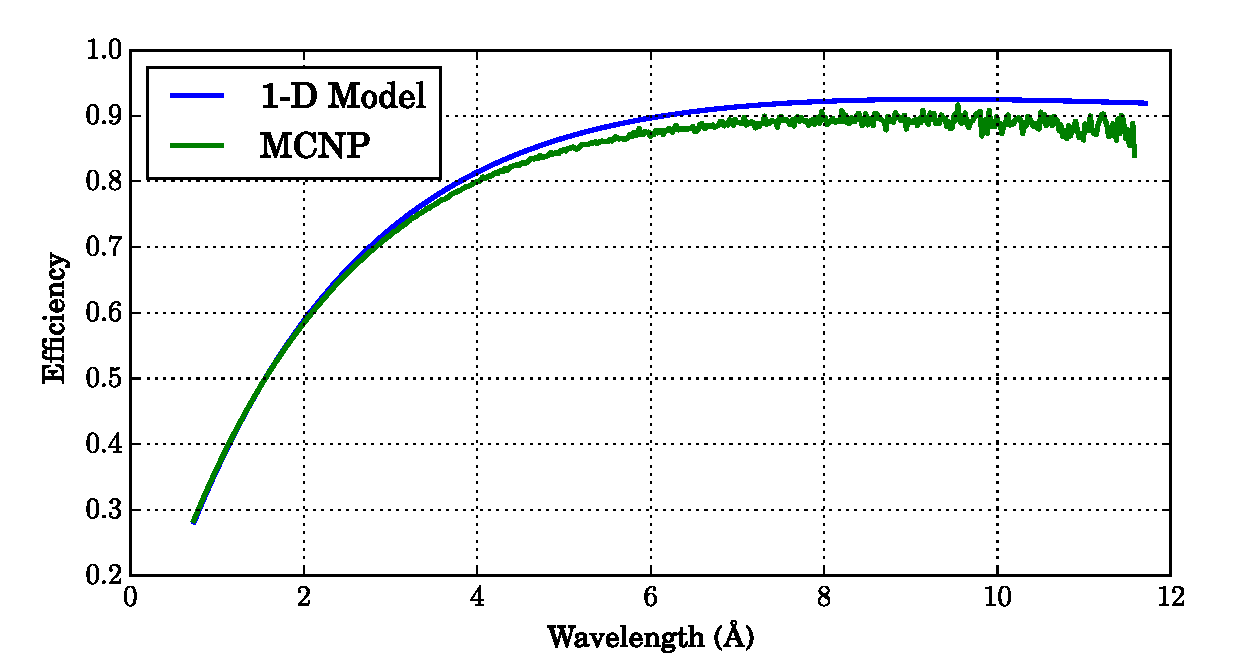
\includegraphics[width=\textwidth]{graphics/eff.eps}
     \caption{The efficiency curves. \label{fig:geom} }
\end{figure}




\section{Measured Brightness}
\label{sec:results}

Five measurements were done in total: centered in the beam port, +20 mm away from center (towards the target), -20 mm away from center (away from the target), centered with beryllium at 77 K in the beamline to show the 4 \AA bin, and without sapphire or beryllium.

\begin{figure}[h!] 
  \centering
    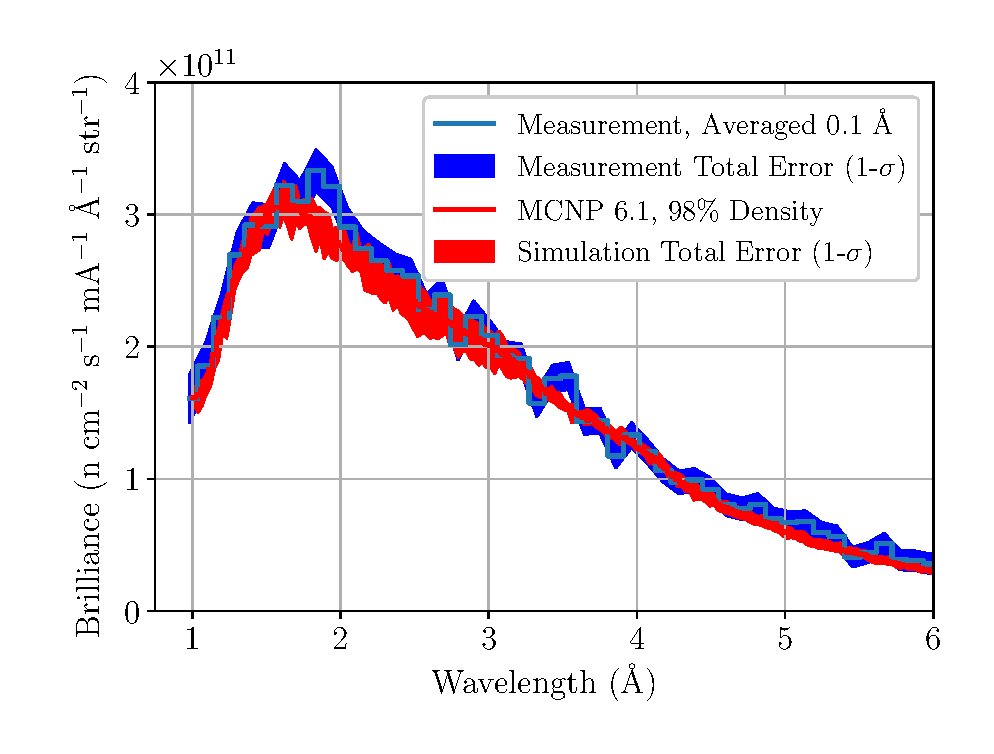
\includegraphics[width=\textwidth]{graphics/brightness.eps}
     \caption{Measured and simulated source brightness at ICON. \label{fig:brightness} }
\end{figure}

\section{Discussion}
\label{sec:discussion}



\section{Conclusions}
\label{sec:conclusions}



\section*{Acknowledgements}
\label{sec:ack}

This work was supported by Swiss National Science Foundation grant 200021\_150048/1


\section*{References}
\bibliographystyle{elsarticle-num-names.bst}
\bibliography{references}

\end{document}

